\documentclass[xcolor=svgnames,t]{beamer} 
\usepackage[utf8]{inputenc}
\usepackage{booktabs, comment}
\usepackage{graphicx}  % Add graphicx package
\usepackage[absolute, overlay]{textpos} 
\usepackage{pgfpages}
\usepackage[font=footnotesize]{caption}
\useoutertheme{infolines} 
\usepackage{xcolor}
% \usepackage{cite}  % REMOVE this line because it conflicts with natbib
\usepackage{colortbl}
\definecolor{brownbrown}{RGB}{8, 8, 9}
\usepackage[round, sort, authoryear]{natbib}  % Use only natbib for citation management
\definecolor{brownred}{RGB}{198, 198, 198}

\setbeamercolor{title in head/foot}{bg=brownred, fg=brownbrown}
\setbeamercolor{author in head/foot}{bg=myuniversity}
\setbeamertemplate{page number in head/foot}{}

\usepackage{amsmath}
\usepackage[makeroom]{cancel}

\newtheorem{equi}{} %Creates a grey box when equi is called
\setbeamertemplate{navigation symbols}{} 
\usepackage{textpos}

\usepackage{tikz}

\usetheme{Madrid}
\definecolor{myuniversity}{RGB}{48, 67, 180}
\usecolortheme[named=myuniversity]{structure}
\usepackage{tikz}


\usepackage{colortbl} 
\newcommand{\myitem}{\item[$\circ$]}
\newcommand{\witem}{\item[\textcolor{white}{$\bullet$}]}
\DeclareMathOperator*{\argmax}{arg\,max}
\DeclareMathOperator*{\argmin}{arg\,min}
\AtBeginSection[]{
\begin{frame}
\frametitle{Content}
\tableofcontents[currentsection]
\end{frame}
}

\title[Causal Regression]{Causal Regression}
\subtitle{}
%\titlegraphic{\includegraphics[height=1cm]{brown-logo.png}}  % This line is commented out to remove the logo
\author[CIML ]{Causal Inference using Machine Learning\\ Master in Economics, UNT}
\institute[]{Andres Mena}
\date{Spring 2024}

\addtobeamertemplate{navigation symbols}{}{%
    \usebeamerfont{footline}%
    \usebeamercolor[fg]{footline}%
    \hspace{1em}%
    \insertframenumber/\inserttotalframenumber
}

\begin{document}
\begin{frame}
\maketitle
\end{frame}

%%%%%%%%%%%%%%%%%%%%%%%%%%%%
%\logo{\includegraphics[height=0.5cm]{brown-arms.png}}  % This line is commented out to remove the logo
%%%%%%%%%%%%%%%%%%%%%%%%%%

\begin{frame}
    \frametitle{Table of Contents}
    \tableofcontents
\end{frame}

\section{Conditional Expectation Function}
\begin{frame}{Definition of CEF}
    \textbf{The Conditional Expectation Function (CEF)}
    \begin{itemize}
        \item The \textit{Conditional Expectation Function (CEF)} is the population average of \( y_i \) given a \( k \times 1 \) vector of covariates \( X_i \), denoted \( E[y_i | X_i] \).
        \pause
        \item For discrete \( y_i \):
        \[
        E[y_i | X_i = x] = \sum_t t P(y_i = t | X_i = x)
        \]
        where \( P(y_i = t | X_i = x) \) is the conditional probability mass function.
        \pause
        \item For continuous \( y_i \):
        \[
        E[y_i | X_i = x] = \int t f_y(t | X_i = x) \, dt
        \]
        where \( f_y(t | X_i = x) \) is the conditional density of \( y_i \) given \( X_i = x \).
        
    \end{itemize}
\end{frame}

\begin{frame}{The Law of Iterated Expectations}
    
       
   
    
    
    \begin{figure}[ht]
        \centering
        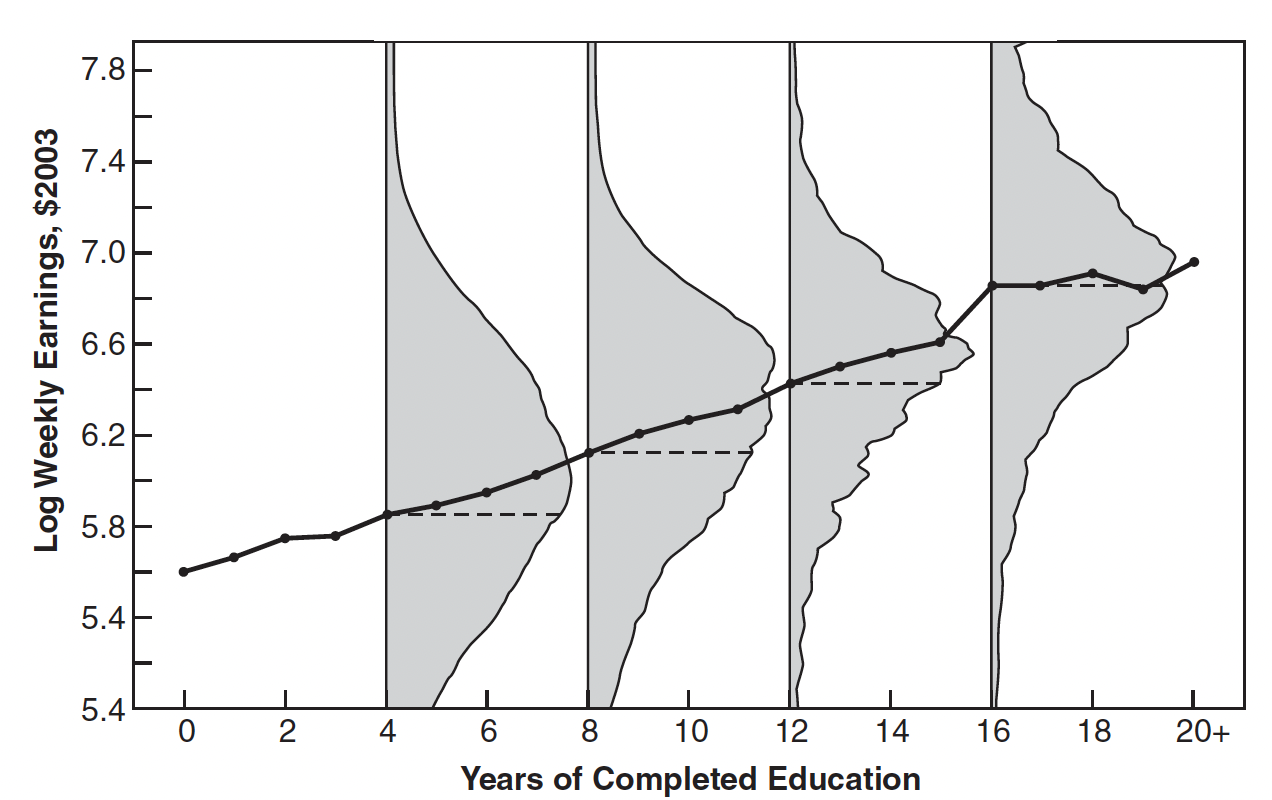
\includegraphics[width=0.7\textwidth]{Figures/CEF.png}
        \caption{CEF of Log Wage on Schooling (Mostly Harmless).}
        \label{fig:cef}
    \end{figure}
    \textbf{LIE:}
    \[
    E[y_i] = E\{E[y_i | X_i]\}
    \]
  
\end{frame}

\begin{frame}{Theorem: The CEF Decomposition Property}
    \textbf{Theorem:}
    \[
    y_i = E[y_i | X_i] + \varepsilon_i
    \]
    \pause
    \begin{itemize}
        \item \( \varepsilon_i \) is the mean independent, i.e \( E[\varepsilon_i]=E[\varepsilon_i | X_i] = 0 \).
        \pause
        \item \( \varepsilon_i \) is uncorrelated with any function of \( X_i \).
    \end{itemize}
    \vspace{1cm}
    \pause
    \textbf{Proof:} i) Replace $\epsilon$, ii) Use LIE to show Orthogonality h(X) and $\epsilon$.
\end{frame}

\begin{frame}{Theorem: The CEF Prediction Property}
    \textbf{Theorem:}
    \[
    E[y_i | X_i] = \arg \min_{m(X_i)} E[(y_i - m(X_i))^2]
    \]
    \begin{itemize}
        \item The CEF \( E[y_i | X_i] \) solves the minimum mean squared error (MMSE) prediction problem.
    \end{itemize}
    \vspace{1cm}
    \textbf{Proof:} Find Normal equations and take conditional expectation.
\end{frame}

\begin{frame}{Theorem: The ANOVA Theorem}
    \textbf{Theorem:}
    \[
    V(y_i) = V(E[y_i | X_i]) + E[V(y_i | X_i)]
    \]
    \begin{itemize}
        \item The total variance equals the variance of the CEF plus the average conditional variance of \( y_i \) given \( X_i \).
    \end{itemize}
    \vspace{1cm}
    \pause
    \textbf{Proof:} Use decomposition property and show $E[\epsilon^2_i]=E[V(y_i | X_i)]$.
\end{frame}

\section{Regression Properties}
\begin{frame}{Regression Problem}
    \textbf{Regression Problem:}
    \[
    \beta_{OLS} = \arg \min_b E[(y_i - X_i b)^2]
    \]
    \begin{itemize}
        \item The vector of population regression coefficients, \(\beta_{OLS}\), is defined as the solution to the population least squares problem.
        \item Using the first-order condition:
        \[
        E[X_i(y_i - X_i b)] = 0
        \]
        \item Solution:
        \[
        \beta_{OLS} = E[X_i X_i']^{-1} E[X_i y_i]
        \]
    \end{itemize}
\end{frame}

\begin{frame}{Linear CEF Theorem}
    \textbf{Theorem:}
    \begin{itemize}
        \item If the CEF is linear, then $X'_i\beta_{OLS}$ is the CEF.

    \end{itemize}
    \vspace{1cm}
    \textbf{Proof:} Assume \( E[y_i | X_i] = X_i' \beta^* \) for any and $\beta^* $,  and show \( \beta_{OLS} = \beta^* \).
\end{frame}

\begin{frame}{Best Linear Predictor (BLP) of Y}
    \textbf{Theorem:}
    \begin{itemize}
        \item The function \( X_i' \beta_{OLS} \) is the best linear predictor of \( y_i \) given \( X_i \) in the MMSE sense.
        
        
    \end{itemize}
    \vspace{1cm}
    \textbf{Proof:} $\beta_{BLP}=\beta_{OLS}$
    \[
        \beta_{BLP} = \arg \min_b E[(y_i - X_i b)^2]
        \]
\end{frame}

\begin{frame}{BLP of the CEF}
    \textbf{Theorem:}
    \begin{itemize}
        \item The function \( X_i' \beta \) provides the MMSE linear approximation to \( E[y_i \mid X_i] \):
        \[
        \beta = \arg \min_b E[(E[y_i \mid X_i] - X_i' b)^2]
        \]
        \item This motivates regression as an approximation to the CEF.
    \end{itemize}
    \vspace{1cm}
    \pause
    \textbf{Proof:} Take conditional expectation of the BLP for Y and note that is the same problem as BLP of the CEF.
\end{frame}

\begin{frame}{Figure: Linear CEF Approximation}
    \textbf{Illustration:}
    \begin{figure}[ht]
        \centering
        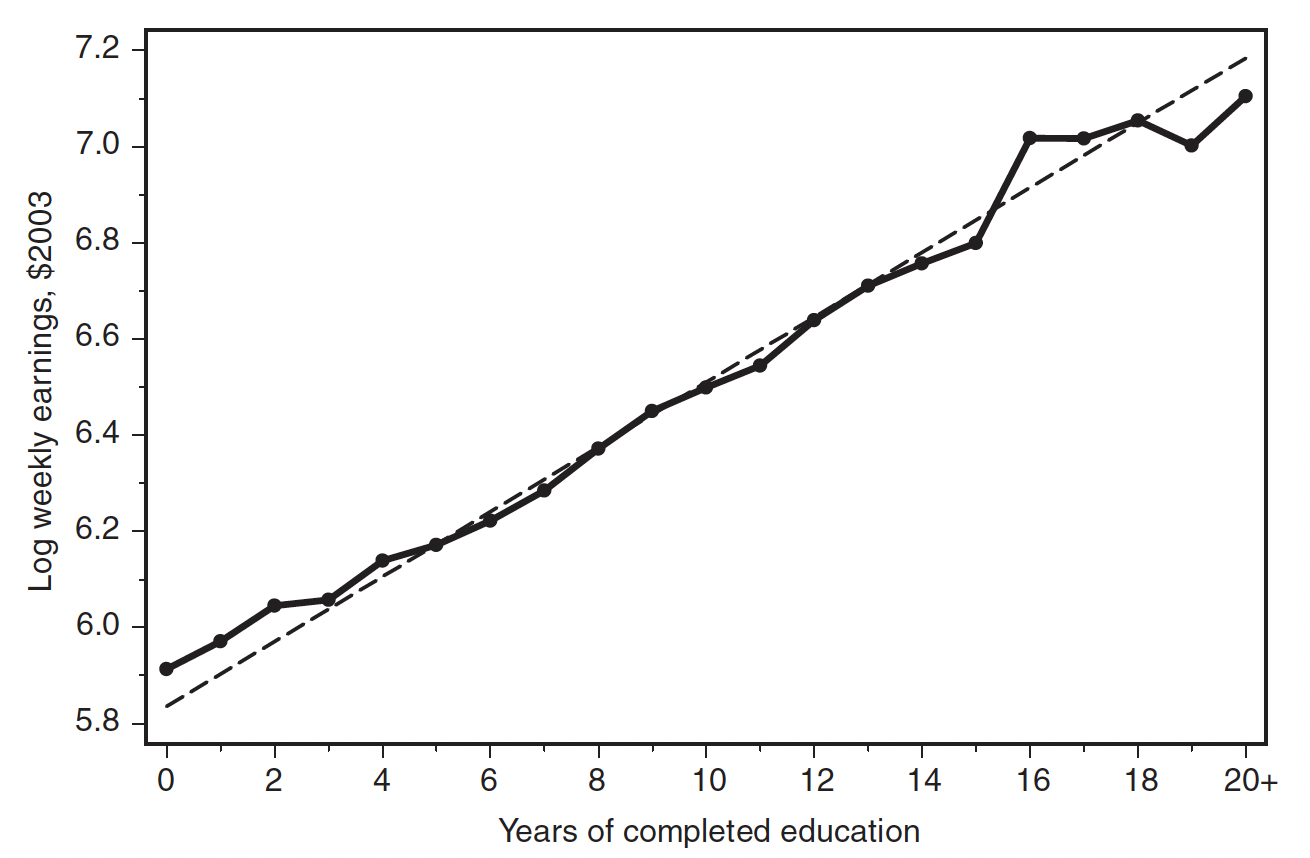
\includegraphics[width=0.8\textwidth]{Figures/Linear_CEF.png}
        \caption{Regression threads the CEF (dots = CEF, dashes = regression line).}
        \label{fig:linear_cef}
    \end{figure}
\end{frame}

\begin{frame}{Bivariate Regression}
    \textbf{Centering:} Subtract the mean of \(X\) and \(Y\) to define centered variables:
    \[
    \tilde{X}_i = X_i - \bar{X}, \quad \tilde{Y}_i = Y_i - \bar{Y}
    \]
    \pause
    \textbf{Centered Regression:}
    \[
    \tilde{Y}_i = \beta_1 \tilde{X}_i + \varepsilon_i
    \]
    \pause
    \textbf{Key Result:}
    The slope coefficient in the centered regression is:
    \[
    \beta_1 = \frac{\sum \tilde{X}_i \tilde{Y}_i}{\sum \tilde{X}_i^2} = \frac{\sum (X_i - \bar{X})(Y_i - \bar{Y})}{\sum (X_i - \bar{X})^2} = \frac{\text{Cov}(Y, X)}{\text{Var}(X)}
    \]
    \pause
    \textbf{Why Center?}
    \begin{itemize}
        \item Simplifies the formula by removing the intercept (\(\beta_0\)).
        \item Directly links \(\beta_1\) to covariance and variance.
        \item Note that \(\bar{X} \to E[X]\) and \(\bar{Y} \to E[Y]\) as \(n \to \infty\).
    \end{itemize}
\end{frame}

\begin{frame}{The Frisch-Waugh-Lovell Theorem}
    \textbf{Theorem: Frisch-Waugh-Lovell (FWL) Theorem}
    \begin{itemize}
        \item In a multivariate regression model, the coefficient of a single variable \(X_k\) in a multiple regression is equivalent to the coefficient obtained by:
        \pause
        \begin{enumerate}
            \item Regressing \(Y\) on all other covariates except \(X_k\), and saving the residuals \( \tilde{Y} \).
            \pause
            \item Regressing \(X_k\) on all other covariates, and saving the residuals \( \tilde{X}_k \).
            \pause
            \item Regressing \( \tilde{Y} \) on \( \tilde{X}_k \).
        \end{enumerate}
    \end{itemize}
    \pause
    \textbf{Key Insight:}  
    The effect of \(X_k\) on \(Y\) can be isolated by removing the influence of other covariates from both \(Y\) and \(X_k\).
\end{frame}

\begin{frame}{Regression Anatomy Formula: Removing estiamted Conditional Expectations under Linearity}
    \textbf{Step 1: Residualizing Variables}
    \begin{itemize}
        \item Define the residualized variables by removing the estimated conditional expectations $\hat{m}(L|X_{-k})$:
        \[
        \tilde{X}_k = X_k - \hat{m}[X_k \mid X_{-k}], \quad \tilde{Y} = Y - \hat{m}[Y \mid X_{-k}]
        \]
        \item This removes the influence of all other covariates (\(X_{-k}\)) on both \(X_k\) and \(Y\), isolating the unique relationship between \(X_k\) and \(Y\).
        \item All the properties of the $CEF$ are preserved, specially the decomposition property.
    \end{itemize}
    \pause
    \textbf{Step 2: Regression on Residualized Variables}
    \[
    \tilde{Y} = \beta_k \tilde{X}_k + \tilde{\varepsilon}
    \]
    \pause
    \textbf{Result:}
    The partial regression coefficient is:
    \[
    \beta_k = \frac{\text{Cov}(Y, \tilde{X}_k)}{\text{Var}(\tilde{X}_k)}
    \]
    
\end{frame}




\section{Causal Regression}

\begin{frame}{Causal Regression Model: Constant Treatment Effect}
    \textbf{Causal Model} $Y_i = Y_i(0) + D_i(Y_i(1) - Y_i(0))$\\
    \pause
    \textbf{Regression Model} $Y_i = \alpha + \beta D_i + \varepsilon_i$
 \pause
    \begin{itemize}
        \item \(\beta\): Constant treatment effect $\beta=Y_i(1)-Y_i(0)$
        \item \(\alpha\): $E[Y_i(0)] $
        \item \(\varepsilon_i\): $Y_i(0)-E[Y_i(0)] $
    \end{itemize}
    \pause
    Show difference between $E[Y_i|D_i=1]$ and $E[Y_i|D_i=0]$
    

   
\end{frame}


\begin{frame}{Regression Coefficient with Covariates (\(\beta\))}

    \textbf{Setup:}
    \[
    Y_i = \beta_0 + \beta D_i + \gamma' X_i + \epsilon_i
    \]
    \pause
    
    
    \pause
    
    Using the regression anatomy formula:
    \[
    \beta = \frac{\text{Cov}(Y_i, \tilde{D}_i)}{\text{Var}(\tilde{D}_i)}, \quad \tilde{D}_i = D_i - \mathbb{E}[D_i | X_i].
    \]
    \pause
    
    \textbf{Expanding the Numerator:}
    \[
    \text{Cov}(Y_i, \tilde{D}_i) = \mathbb{E}[(D_i - \mathbb{E}[D_i | X_i]) Y_i].
    \]
    \pause
    
    By the Law of Iterated Expectations (LIE), substitute \(Y_i\) with \(\mathbb{E}[Y_i | D_i, X_i]\). \textbf{Define CATE:}
    \(
    \tau(X_i) = \mathbb{E}[Y_i(1) - Y_i(0) | X_i].
    \)
    \[
    \mathbb{E}[Y_i | D_i, X_i] = \mathbb{E}[Y_i | D_i = 0, X_i] + \tau(X_i) D_i.
    \]
    
    \end{frame}
    

    \begin{frame}{Regression Coefficient with Covariates}

        \textbf{Decomposing the Covariance:}
        \[
        \mathbb{E}\big[(D_i - \mathbb{E}[D_i | X_i]) \mathbb{E}[Y_i | D_i = 0, X_i]\big] + \mathbb{E}\big[(D_i - \mathbb{E}[D_i | X_i]) \tau(X_i) D_i\big]
        \]
        \pause
        - The first term vanishes (why?)\\
        \pause
        - The second term simplifies:
        \[
        \mathbb{E}[(D_i - \mathbb{E}[D_i | X_i]) D_i \tau(X_i)] = \mathbb{E}[(D_i - \mathbb{E}[D_i | X_i])^2 \tau(X_i)].
        \]
        
        \pause
        \textbf{Final Expression:}
        \[
        \beta = \frac{\mathbb{E}[(D_i - \mathbb{E}[D_i | X_i])^2 \tau(X_i)]}{\mathbb{E}[(D_i - \mathbb{E}[D_i | X_i])^2]}.
        \]
        
        \pause
        \textbf{Weighted Average:}
        Define \(\sigma^2_D(X_i) = \mathbb{E}[(D_i - \mathbb{E}[D_i | X_i])^2 | X_i]\). Then:
        \[
        \beta = \frac{\mathbb{E}[\sigma^2_D(X_i) \tau(X_i)]}{\mathbb{E}[\sigma^2_D(X_i)]}.
        \]
        
        \textbf{Conclusion:}
        - \(\beta\) is a variance-weighted average of CATE \(\tau(X_i)\).
        - The weights depend on the conditional variance of \(D_i\) given \(X_i\).
        
        \end{frame}
        
        



\section{Inference in Regression}

\begin{frame}{Classical Additive Approach - Population Setup}

    \textbf{Population Linear Projection:}
    \[
    Y = D \beta + X' \gamma + \epsilon, \quad \epsilon \perp (D, X),
    \]
    where:
    \begin{itemize}
        \item \(D\) is the treatment indicator,
        \item \(X = (1, W)\) includes an intercept and covariates with \(\mathbb{E}[W] = 0\),
        \item \(D \perp W\) (randomized controlled trial).
    \end{itemize}
    
    \textbf{Key Results:}
    - Decompose \(\gamma' X = \gamma_1 + \gamma_2' W\).
    - For \(U := \gamma_2' W + \epsilon\):
      \[
      Y = D \beta + \gamma_1 + U, \quad U \perp (1, D).
      \]
    
    \textbf{Interpretation of Coefficients:}
    - \(\beta = \mathbb{E}[Y(1)] - \mathbb{E}[Y(0)]\) (ATE),
    - \(\gamma_1 = \mathbb{E}[Y(0)]\) (average untreated outcome).
    
    \end{frame}
    

    \begin{frame}{Projection Properties}

        \textbf{Projection Setup:}
        \[
        Y = D \beta + \gamma_1 + U, \quad U \perp (1, D).
        \]
        
        \textbf{Key Implications:}
        - The population projection of \(Y\) onto \((1, D)\) yields:
          \[
          Y = \mathbb{E}[Y | D] = D \beta + \gamma_1.
          \]
        - The coefficients \((\beta, \gamma_1)\) are the same as those obtained by the two-sample approach in the population:
          \[
          \beta = \mathbb{E}[Y(1)] - \mathbb{E}[Y(0)], \quad \gamma_1 = \mathbb{E}[Y(0)].
          \]
        
        \textbf{RCT Setting:}
        - Randomization ensures:
          \[
          D \perp W, \quad \epsilon \perp (D, W).
          \]
        
        \end{frame}
        
           
        \begin{frame}{Approximate Normality of \(\hat{\beta}\)}

            \textbf{OLS Estimator for \(\beta\):}
            \[
            \sqrt{n} (\hat{\beta} - \beta) \approx \sqrt{n} \frac{\mathbb{E}_n[\epsilon \tilde{D}]}{\mathbb{E}_n[\tilde{D}^2]} \sim \mathcal{N}(0, V_{11}),
            \]
            where:
            \begin{itemize}
                \item \(\tilde{D} = D - \mathbb{E}[D | X]\) (residual after partialling out \(X\)),
                \item \(V_{11} = \frac{\mathbb{E}[\epsilon^2 \tilde{D}^2]}{(\mathbb{E}[\tilde{D}^2])^2}\).
            \end{itemize}
            
            \textbf{Key Derivation Steps:}
            1. Partial out \(X = (1, W)\) from \(D\),
            2. Use OLS theory to approximate the distribution of \(\hat{\beta}\).
            
            \end{frame}
            
            \begin{frame}{Approximate Normality of \(\hat{\gamma}_1\) and Joint Properties}

                \textbf{OLS Estimator for \(\gamma_1\):}
                \[
                \sqrt{n} (\hat{\gamma}_1 - \gamma_1) \approx \sqrt{n} \frac{\mathbb{E}_n[\epsilon \tilde{1}]}{\mathbb{E}_n[\tilde{1}^2]} \sim \mathcal{N}(0, V_{22}),
                \]
                where:
                \begin{itemize}
                    \item \(\tilde{1} = 1 - \mathbb{E}[1 | D, X]\) (residual after partialling out \(D\) and \(X\)),
                    \item \(V_{22} = \frac{\mathbb{E}[\epsilon^2 \tilde{1}^2]}{(\mathbb{E}[\tilde{1}^2])^2}\).
                \end{itemize}
                
                \textbf{Joint Normality:}
                The estimators \(\hat{\beta}\) and \(\hat{\gamma}_1\) are jointly normal:
                \[
                \text{Cov}(\hat{\beta}, \hat{\gamma}_1) \sim V_{12},
                \]
                where:
                \[
                V_{12} = \frac{\mathbb{E}[\epsilon^2 \tilde{D} \tilde{1}]}{\mathbb{E}[\tilde{D}^2] \mathbb{E}[\tilde{1}^2]}.
                \]
                
                \end{frame}
                
       


    


\end{document}


































 


